\section{Recurrent Neural Networks}
\label{sec:rnn}
Recurrent Neural Networks (RNNs) are one of the most commonly used typology of neural networks~\cite{lecun2015deep}. In recent years, thanks to advancements in their architecture~\cite{hochreiter1997long,chung2014empirical} and in computational power, they have become the standard to effectively model sequential data. They have been used successfully for tasks such as sentiment analysis~\cite{tang2015document}, speech recognition~\cite{graves2013speech}, image captioning~\cite{karpathy2015deep}, predicting tourist paths~\cite{palumbo2017predicting} and neural language models~\cite{mikolov2010recurrent}. One of the typical applications of RNNs is language modeling, i.e. the task of learning a probabilistic model of text in order to generate new text by recursively predicting the next word in a sentence~\cite{sutskever2011generating}. We use RNNs, more specifically Long-Short Term Memory (LSTM) cells~\cite{hochreiter1997long}, in a similar vein to the language modeling problem, i.e. training the network to predict the next track in a playlist and sampling tracks from the learned probability model to generate predictions. In practice, rather than using only the track as input, we use a richer representation that also exploits the artist, the album, the title and, possibly, lyrics features (Figure~\ref{fig:global_architecture}). 

In the following sections, we describe in detail the input features as well as the generation strategy.

\begin{figure*}
    \centering
    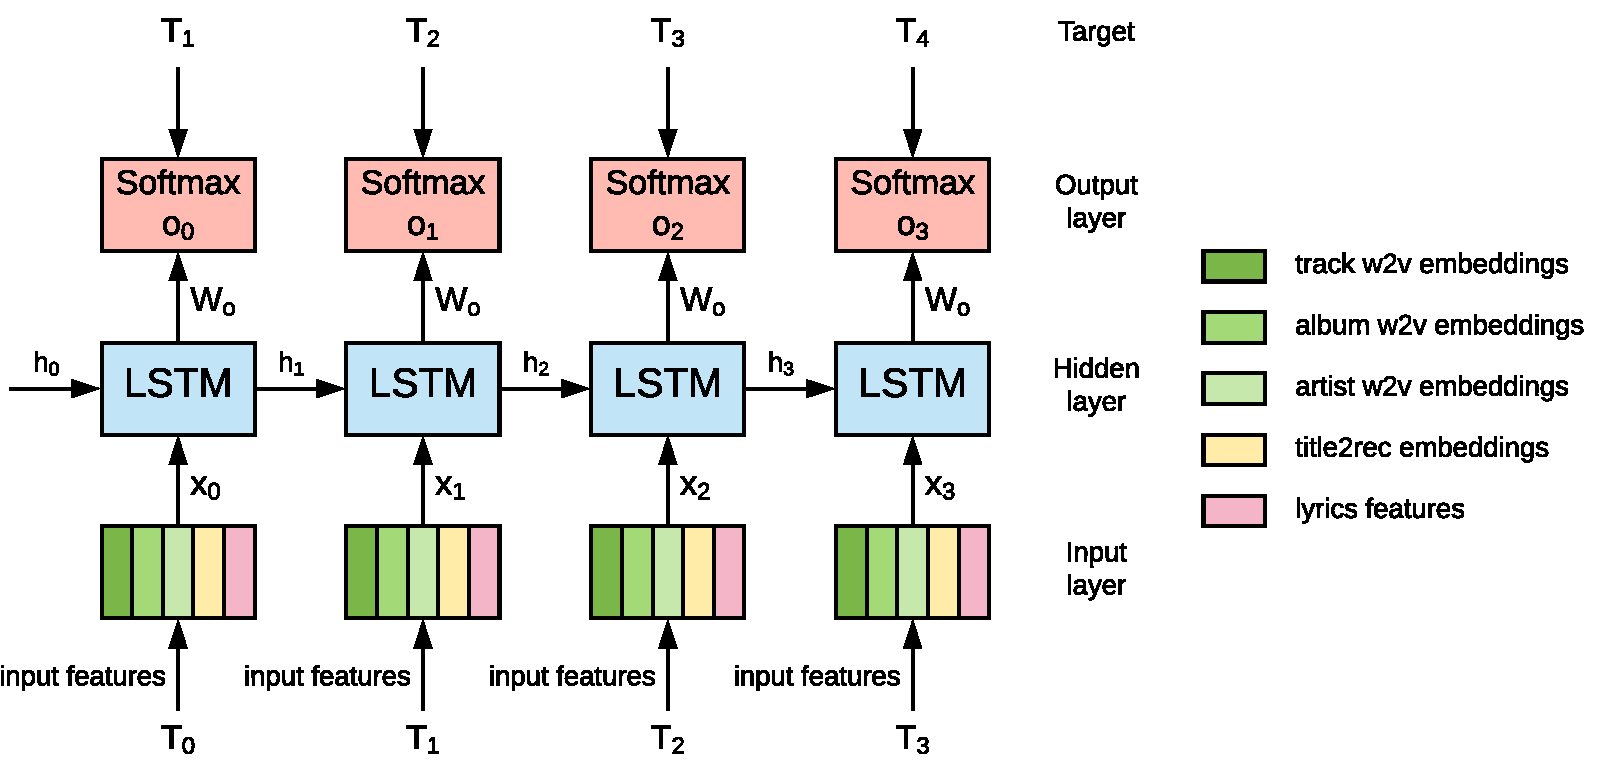
\includegraphics[width=0.7\textwidth, height=0.35\textwidth]{figures/rnn.pdf}
    \caption{RNN architecture for playlist completion. The input vectors include word2vec embeddings for the track, the album, and the artist, a fastText embedding for the playlist title and numerous features extracted from the lyrics.}
    \label{fig:global_architecture}
\end{figure*}

\subsection{Input Vectors}

\subsubsection{Track, Album and Artist Embeddings}
\label{sec:track_embs}
In order to leverage the information in the dataset concerning tracks, artists and albums, we opt for an approach based on word2vec~\cite{mikolov2013distributed} embeddings. More precisely, we train the word2vec model separately on sequences of tracks, albums and artists in the order of appearance in the playlist, obtaining three separated word2vec models encoding co-occurrence patterns of tracks, albums and artists respectively. Each word2vec model is based on the Skip-gram model with negative sampling using default hyper-parameters of the Gensim implementation~\cite{rehurek_lrec}: embedding vector dimension is $d=100$, learning rate $\alpha = 0.025$ linearly decaying up to $min_{\alpha} = 0.0001$, window size $c = 5$, number of epochs is $\eta = 5$.

We concatenate the three representations of the tracks, albums and artists, obtaining an input vector $x_{w2v}$ whose dimensionality is $|x_{w2v}| = 300$.

\subsubsection{Titles Embeddings}
\label{sec:title_embs}
The title of a playlist can potentially contain interesting information about the intention and the purpose of its creator. The title can suggest that the tracks in certain playlist are intended to suit a certain goal (e.g. \textit{party}, \textit{workout}), a mood (\textit{sad songs}, \textit{relaxing}), a genre (\textit{country}, \textit{reggae}), or a topic (\textit{90's}, \textit{Christmas}). Our intuition, supported by the experiments described later in this section, is that playlists with similar titles may contain similar tracks.
The title similarity could rely on pre-trained models and thesauri. However, we opted for computing a model that is specific for the playlist continuation task, using the sole data of the MPD.

A playlist embedding $p_{w2v}$ is computed as the mean of the embeddings of the tracks composing the playlist, already generated in Section \ref{sec:track_embs}. The playlist embeddings are then grouped in $n$ clusters, applying the K-means algorithm.

We empirically observed that, apart from very general clusters, we also created clusters containing specialized playlists, obtaining as a consequence groups of titles that belong to the same semantic area. For example, a cluster contains playlists like \textit{Christmas feels}, \textit{December} or with titles including the emoji of Santa Claus, while another group encompasses playlists like \textit{country} and \textit{Alabama}.

Each cluster $c$ expresses a composed label, which is the concatenation of the titles of all the playlist $p \in c$ separated by a blank space. These labels can be seen as a corpus of $n$ documents (one for each cluster) that is used as input for the fastText algorithm~\cite{joulin2016fasttext}. Because this algorithm is able to represent textual information at the level of n-grams from 3 to 6 character, the Title2Rec model in output computes the embeddings of any playlist title, being this already seen in the dataset or totally unknown. Figure~\ref{fig:t2r_pipeline} illustrates the process of the Title2Rec model generation.

% source: https://docs.google.com/presentation/d/1KV4eFuYvFxS1Z25ZwOqu5TJ2zuBbeRAZAkR2Hbf8h_A/edit#slide=id.g3d7920112c_0_0
\begin{figure*}
    \centering
    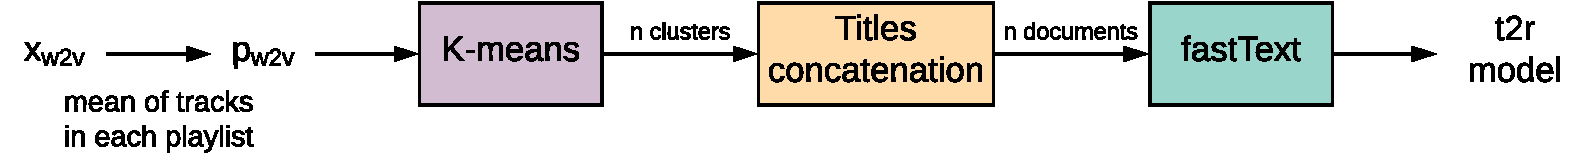
\includegraphics[width=0.85\textwidth]{figures/t2r.pdf}
    \caption{Pipeline for generating the title embedding model used in Title2Rec. The embeddings are computed through a fastText model trained on a corpus of concatenated titles of similar playlists.}
    \label{fig:t2r_pipeline}
\end{figure*}

\subsubsection{Lyrics Embeddings}
\label{sec:lyrics}
Since playlists contain tracks that share semantic properties (such as the genre) and acoustic properties (such as the mood), we hypothesize their lyrics share features as well. To this end, we extract numerous features from the lyrics for a large set of tracks used in the MPD dataset ($v \in \mathbb{R}^{n}$) that describe different stylistic and linguistic dimensions of a song text:
\begin{itemize}
  \item \textit{vocabulary} ($v \in \mathbb{R}$): as a measure of the vocabulary richness, we compute the type-token ratio of a song text.
  \item \textit{style} ($v \in \mathbb{R}^{27}$): to estimate the linguistic style of a song text, we measure the line lengths (in characters and in tokens) and the frequencies of all major part-of-speech tags. We further count rhyme occurrences and \qu{echoisms} (sung words like \qu{laaalala} and \qu{yeeeeeeeaaaaaaah}).
  \item \textit{semantics} ($v \in \mathbb{R}^{60}$): we build a topic model with 60 topics on the song text bag of words using Latent Dirichlet Allocation~\cite{LDA}. Each song text is then represented by its association to these topics.
  \item \textit{orientation} ($v \in \mathbb{R}^{3}$): this dimension models how the song narrative (entities, events) is oriented with respect to the world. We encode a temporal dimension, i.e. whether the song mainly recounts past experiences or present/future ones, by representing the fraction of past tense verb forms to all verb forms as a feature.
  \item \textit{emotion} ($v \in \mathbb{R}^{6}$): we model the subjectivity (subjective vs. objective) as well as the polarity (positive vs. negative) of the song text. Furthermore, the emotions conveyed are modelled in a common two-dimensional model that accounts for degrees of arousal and valence.
  \item \textit{song structure} ($v \in \mathbb{R}^{4}$): as a proxy of the structure of the lyrics, we use the line lengths as well as the lengths of paragraphs in the song text.
\end{itemize}

For experimental purposes, we grouped the previous features in two additional categories:
\begin{itemize}
    \item \textit{deterministic} ($v \in \mathbb{R}^{23}$): it encompasses all features generated in a deterministic way such as features related to the structure, the vocabulary, and the style of the lyrics. We excluded from this group the frequencies of part-of-speech tags, as they depend on the tagger used.
    \item \textit{fuzzy} ($v \in \mathbb{R}^{18}$): it includes the features generated in a non-deterministic fashion such as orientation, emotion, and the frequencies of part-of-speech tags.
\end{itemize}

All features are scaled using a custom feature scaler that combines two elements: i) account for outliers by scaling the data non-linearly based on the percentile of the feature value distribution they belong to; ii) scale the data linearly to the same $[-1,1]$ interval that non-lyrics features live in.

Retrieving lyrics for the MPD dataset is achieved by linking it to the WASABI corpus~\cite{meseguerbrocal:hal-01589250}.\footnote{\url{https://wasabi.i3s.unice.fr}} The WASABI corpus is an ongoing resource that contains 2.1M song texts (of 77k artists), and for each song it provides the following information: the lyrics extracted from \url{http://lyrics.wikia.com}, the synchronized lyrics (when available) from \url{http://usdb.animux.de}, DBpedia abstracts and categories the song belongs to, genre, label, writer, release date, awards, producers, artist and/or band members, the stereo audio track from Deezer (when available), the unmixed audio tracks of the song, its ISRC, BPM, and duration. In total, we linked 416k tracks in MPD (out of 2.2M unique tracks) to WASABI tracks that contain the lyrics. While the linked tracks proportion with $\sim$20\% seems small, the linked tracks cover 53\% of all 66M track occurrences in MPD because of the typical fat-tailed distribution, where some songs are extremely common while most titles occur only rarely in a playlist. Linking the lyrics was done in three levels of accuracy: direct Spotify URI matching gave us 155k links, exact artist and title matching provided 334k matches, and finally lower casing and deleting bracketed content (in song titles only) led to 51k matches. As the results overlap we ended up with 416k matched tracks in total. Some of our lyrics features are language-specific, so we decided to compute lyrics features exclusively on English song texts. This finally resulted in 367k English song texts we computed lyrical features on. Language detection is done with the \textit{langdetect} package\footnote{\url{https://github.com/Mimino666/langdetect}} and datasets of MPD and WASABI are merged along the axes of their Spotify URIs, artist names, song title names, respectively.

\subsection{Learning Model}
As mentioned earlier, we address the problem of playlist continuation as a language modeling problem. More specifically, we train the RNN to predict the next track in a playlist, defining the targets $Y$ to be the inputs $X$ shifted in time, i.e. $X = \{(\hat{T{^j}}_0, \hat{T{^j}}_1, \dots, \hat{T^{j}}_{N_j -1})\}$ and $Y = \{(T{^j}_1, T{^j}_2, \dots, T^{j}_{N_j})\}$ where $\hat{T}$ represents a track and its metadata (artist, album, playlist title, lyrics features), $T$ represents a track id in a playlist, $j = 1, \dots, M$ is a playlist index and $N_j$ is the length of the j-\textit{th} playlist. In this way, we train the model to learn a probability distribution of the next track $P (T_N | \hat{T}_{N-1}, \hat{T}_{N-2}, \dots, \hat{T}_{0})$ given the previous ones, which is parametrized by the network outputs that are converted into probabilities by the final softmax layer (Figure~\ref{fig:global_architecture}). The training algorithm attempts to minimize the cross-entropy loss function $L$, that measures the disagreement between the learned probability model and the observed probability model of the targets $Y$. The perplexity metric that is reported in the experiments (Section~\ref{sec:rnn-opt}) corresponds to $ppl = 2^{L}$. In practice, rather than using probabilities, we use the `logits' $p_i$ where $i$ is a track index, un-normalized scores that are proportional to the probabilities. Different optimization algorithms to minimize the loss are empirically compared (Section~\ref{sec:rnn-opt}).

\subsection{Generating predictions}
\label{sec:generation}
We experiment three different strategies to generate track predictions from the RNN. Given an input seed and the hidden state, the trained model outputs the logits $p_i$, i.e. un-normalized scores that are proportional to the probability that a given track appears after the sequence of seeds $s$. In details, we considered the following approaches, as depicted in Figure~\ref{fig:predictions}.
\begin{description}
    \item[do\_sample] It samples the track with the highest logit $p_i$, where $\hat{i} = arg\ max ({p_i})$, given the set of seeds $s$. It adds the sampled track $\hat{i}$ to the seeds $s$, then it repeats the previous operations until 500 tracks are sampled.
    \item[do\_rank] It ranks the tracks according to their logit value $p_i$, given all the seeds $s$, then it selects the top-500 tracks with the highest logit.
    \item[do\_summed\_rank] It computes the logits $p_i$ for every seed. It averages all the logits in the sequence obtaining $\hat{p_i}$ and then it ranks the tracks according to the values of $\hat{p_i}$.
\end{description}

\begin{figure}
	\centering
	\begin{subfigure}{0.4\textwidth}
		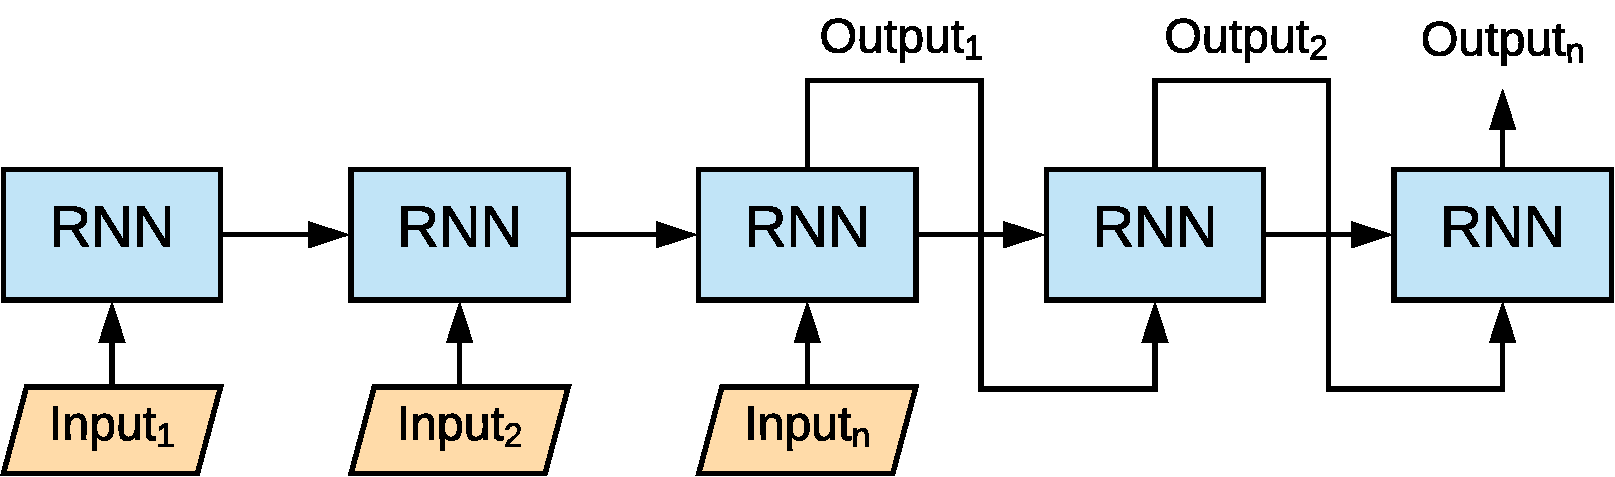
\includegraphics[width=\textwidth]{figures/sample.pdf}
		\caption{do\_sample}
	\end{subfigure}
	\begin{subfigure}{0.4\textwidth}
		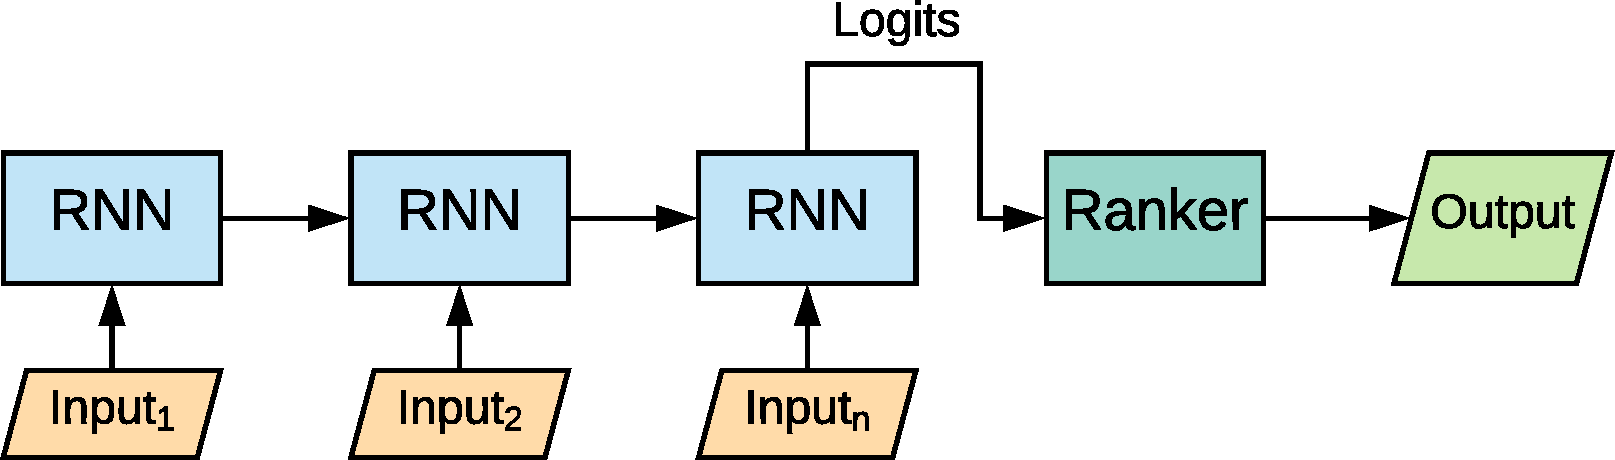
\includegraphics[width=\textwidth]{figures/rank.pdf}
		\caption{do\_rank}
	\end{subfigure}
	\begin{subfigure}{0.4\textwidth}
		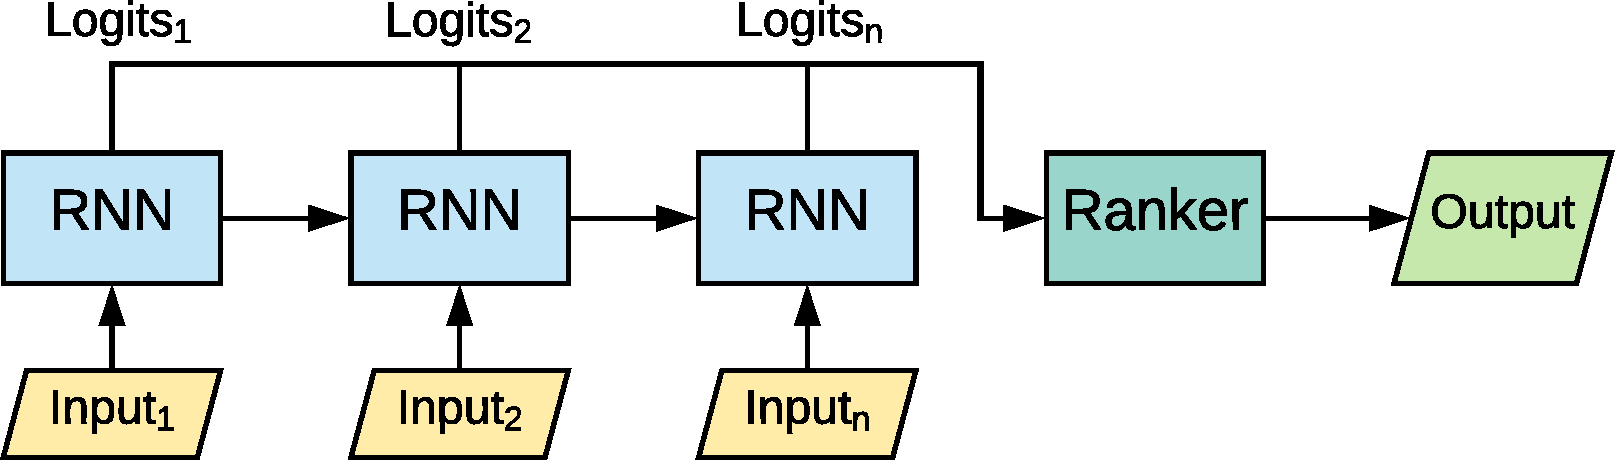
\includegraphics[width=\textwidth]{figures/summed.pdf}
		\caption{do\_summed\_rank}
	\end{subfigure}
	\caption{Three strategies for generating track predictions.}
	\label{fig:predictions}
\end{figure}
